\documentclass[12pt]{article}
\usepackage{amsmath}
\usepackage{graphicx}
\usepackage{fancyhdr}
\usepackage{geometry}
\usepackage{float}
\usepackage{longtable}
\geometry{a4paper}

\title{Cerberus: Federated Learning (FL) setup implemented in C}
\author{Lakshay Chauhan, Chaitanya Arora}
\date{December 1, 2024}

\begin{document}
	
	\maketitle
	
	\noindent \textit{For code specification please look at \(report/CODE\_SPECIFICATION.pdf\).}
	\\

	\noindent Parameters used to obtain the further mentioned results, the aforementioned parameters are taken from the file \(report/params.config\).
		
	\begin{table}[h!]
		\centering
		\begin{tabular}{|l|l|p{8cm}|}  % 8cm width for the description column
			\hline
			\textbf{Parameter}         & \textbf{Value}      & \textbf{Description}  \\ \hline
			input\_size                & 784                 & The number of input features (e.g., for MNIST, it represents 28x28 pixel images). \\ \hline
			hidden\_size               & 128                 & The number of neurons in the hidden layer of the neural network. \\ \hline
			output\_size               & 10                  & The number of output classes (e.g., for MNIST, it represents 10 digits). \\ \hline
			port                       & 3000                & The port number used for communication or networking. \\ \hline
			learning\_rate             & 0.01                & The learning rate for training the model, controlling the step size during optimization. \\ \hline
			local\_epochs              & 10                  & The number of epochs (iterations over the dataset) to train the model on each client locally. \\ \hline
			log\_train\_metrics        & 1                   & A flag (1 or 0) to enable or disable logging of training metrics during training. \\ \hline
			num\_clients               & 3                   & The number of clients participating in a distributed training setup. \\ \hline
			global\_epochs             & 10                  & The number of global epochs (iterations over the dataset) for the overall training process. \\ \hline
		\end{tabular}
		\caption{Parameters configuration and description}
		\label{tab:config_parameters}
	\end{table}
	
	\begin{figure}
		\centering
		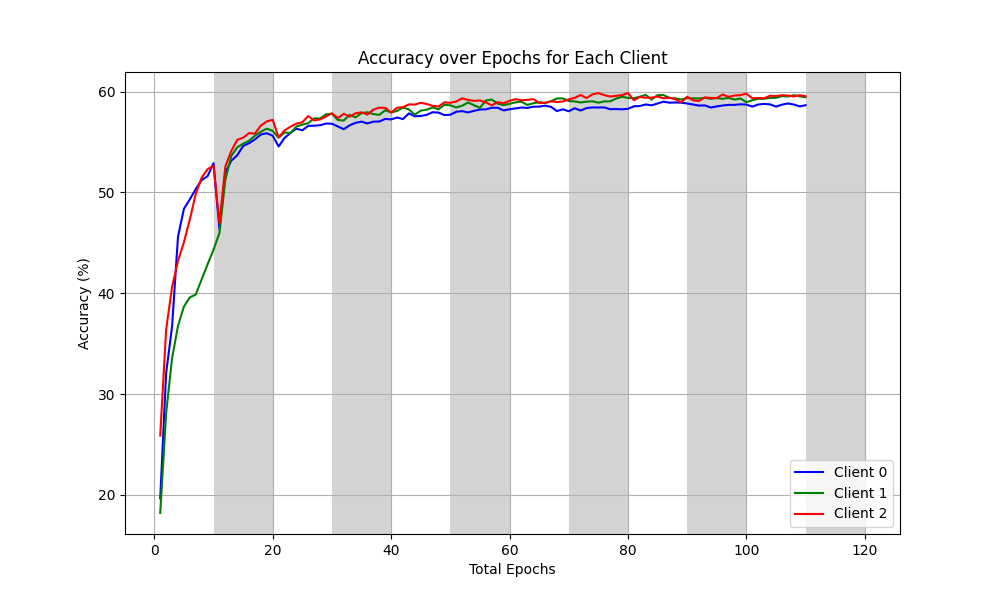
\includegraphics[width=\linewidth]{acc_vs_epoch}
		\caption{Accuracy vs Epoch plot for all the clients. The gray white blocks define the transition from one global epoch to another.}
		\label{fig:acc_vs_epoch}
	\end{figure}
	
	\begin{figure}
		\centering
		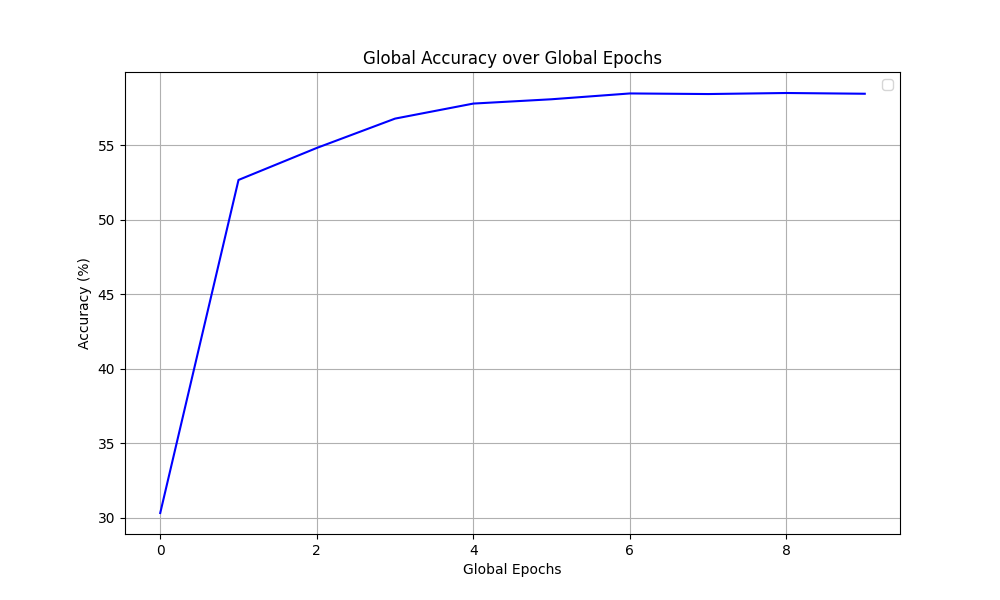
\includegraphics[width=\linewidth]{global_acc_vs_epoch}
		\caption{Global Accuracy vs Global Epoch plot}
		\label{fig:global_acc_vs_epoch}
	\end{figure}
	
\end{document}
